%!TEX root=/Users/sergej/Documents/Master/Thesis/main.tex
\section{Ranking of structural Ricardian comparative advantage }
In this section I present the results of the structural RCA ranking for both value-added exports measures and gross exports.
I will give two views on the structural RCA ranking a global view and a local view.
First, the global view will shows a scatter plot of the association of the RCA ranking for gross exports and value-added exports and a country's per capita GDP.
The global view investigates the hypothesis that country's with a higher GDP show a higher similarity between the rankings and hence their sourcing and factor usage are not strongly sector specific. \par
Second, the local view focuses on comparing the structural RCA ranking for Belgium and Germany of forward and backward value-added exports to gross exports.
In this way, I analyze two aspects, first whether value-added exports alter the picture of comparative advantage and whether the different perspectives of value-added exports affect the results.
\subsection{Structural Ricardian comparative advantage based gross exports and value-added exports}
I will discuss the choice of the association measures shortly.
First of all, I chose the Spearman's $\rho$  since I focus on the similarity of the rankings and the strength of the monotonic association between them.
Moreover I chose Kendall's $\tau$ as it computes the similarity of the two rankings, by the means of counting the number of country pairs, which are different between two rankings.% Concretely, for each draw of country pairs I record in a binary variable, whether the draws are of the same order as in the ordered set. The binary variable is equal to one if the order is the same and zero else. In the next step I compute a simple correlation coefficient on the set of binary variables.
\par
I outline the construction of Kendall's $\tau$ based on \textcite{abdi2007kendall}.
The outline makes the simple interpretation of Kendall's $\tau$ in terms of probabilities more clear.
The basic idea behind the measure is to count the number of different pairs of two sets of ordered  objects, which include the same objects  \textcite{abdi2007kendall}.
I illustrate this idea in the context of the RCA rankings.
For two RCA rankings, the measure is based on counting the number of different ordered country pairs, which I denote as $d(P_1, P_2)$, where $P_i \quad i=1,2$ indicates the two ordered set of pairs obtained from the country rankings.
In the next step, this number is normalized such that is bounded by -1 and 1, where -1 reflects the largest differences and 1 is equal to the smallest difference.
Kendall's $\tau$ is then defined as follows \[ \tau= \frac{1/2 N(N-1) - d(P_1,P_2)} {1/2 N(N-1)} .\] %where the nominator $1/2 N(N-1)$ is equal to the number of pairs one can obtain from a set of $n$ objects.
Moreover, Kendall's $\tau$ has an intuitive stochastic interpretation based on the idea of drawing orderd pairs \parencite{abdi2007kendall}.
In the context of two country rankings, the interpretation is that if a country pair is randomly drawn from each ranking, Kendall's $\tau$ is the difference between the probability that the draws have the same order and the probability that the country pairs have a different order.
The focus of Kendall's $\tau$ on country pairs is especially useful for RCA, as the main focus of RCA is to compare pairs of countries and industries.   \par
\begin{figure}[H]
\caption{Association RCA based on VAX \& EXGR and GDP per capita }
\centering
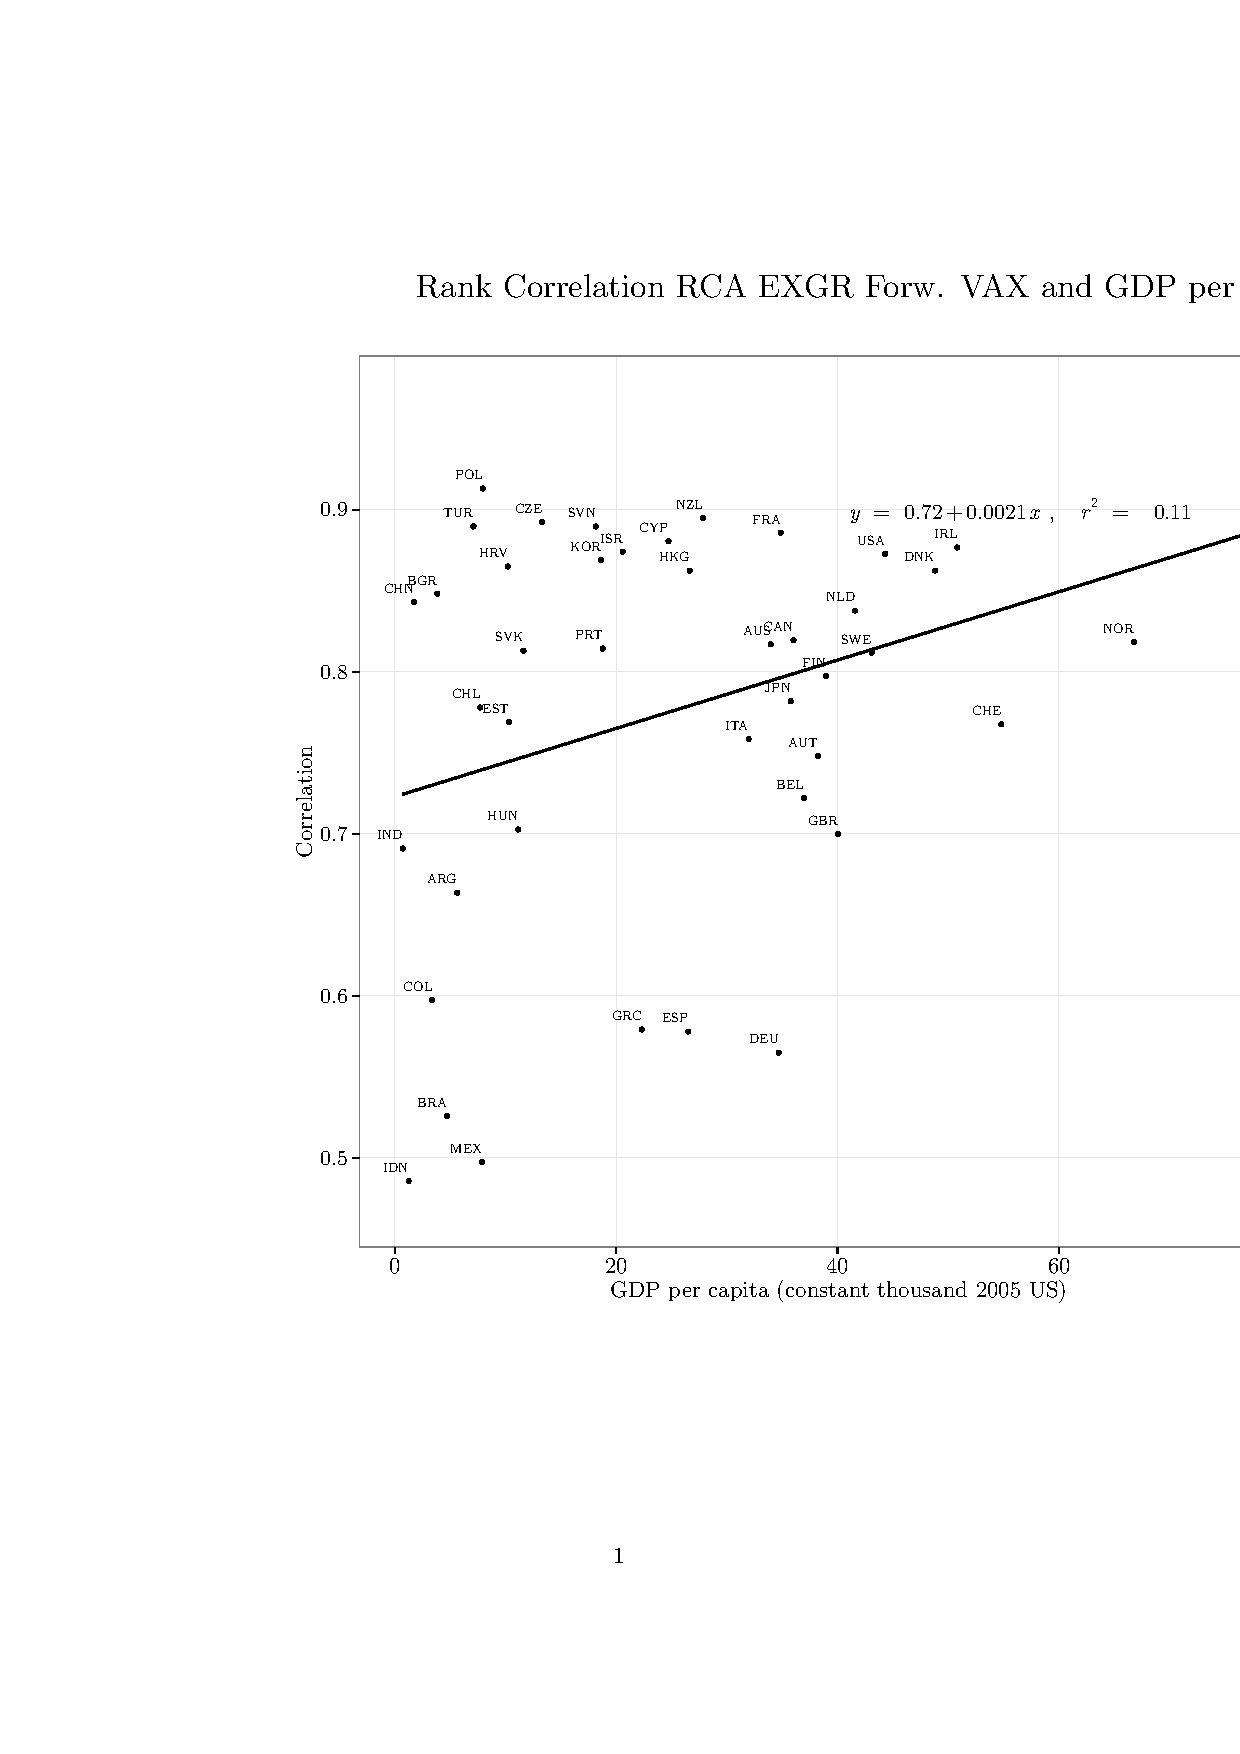
\includegraphics[width=.49 \linewidth]{./fig/spearman_fddva_std_balassa-march.tex}
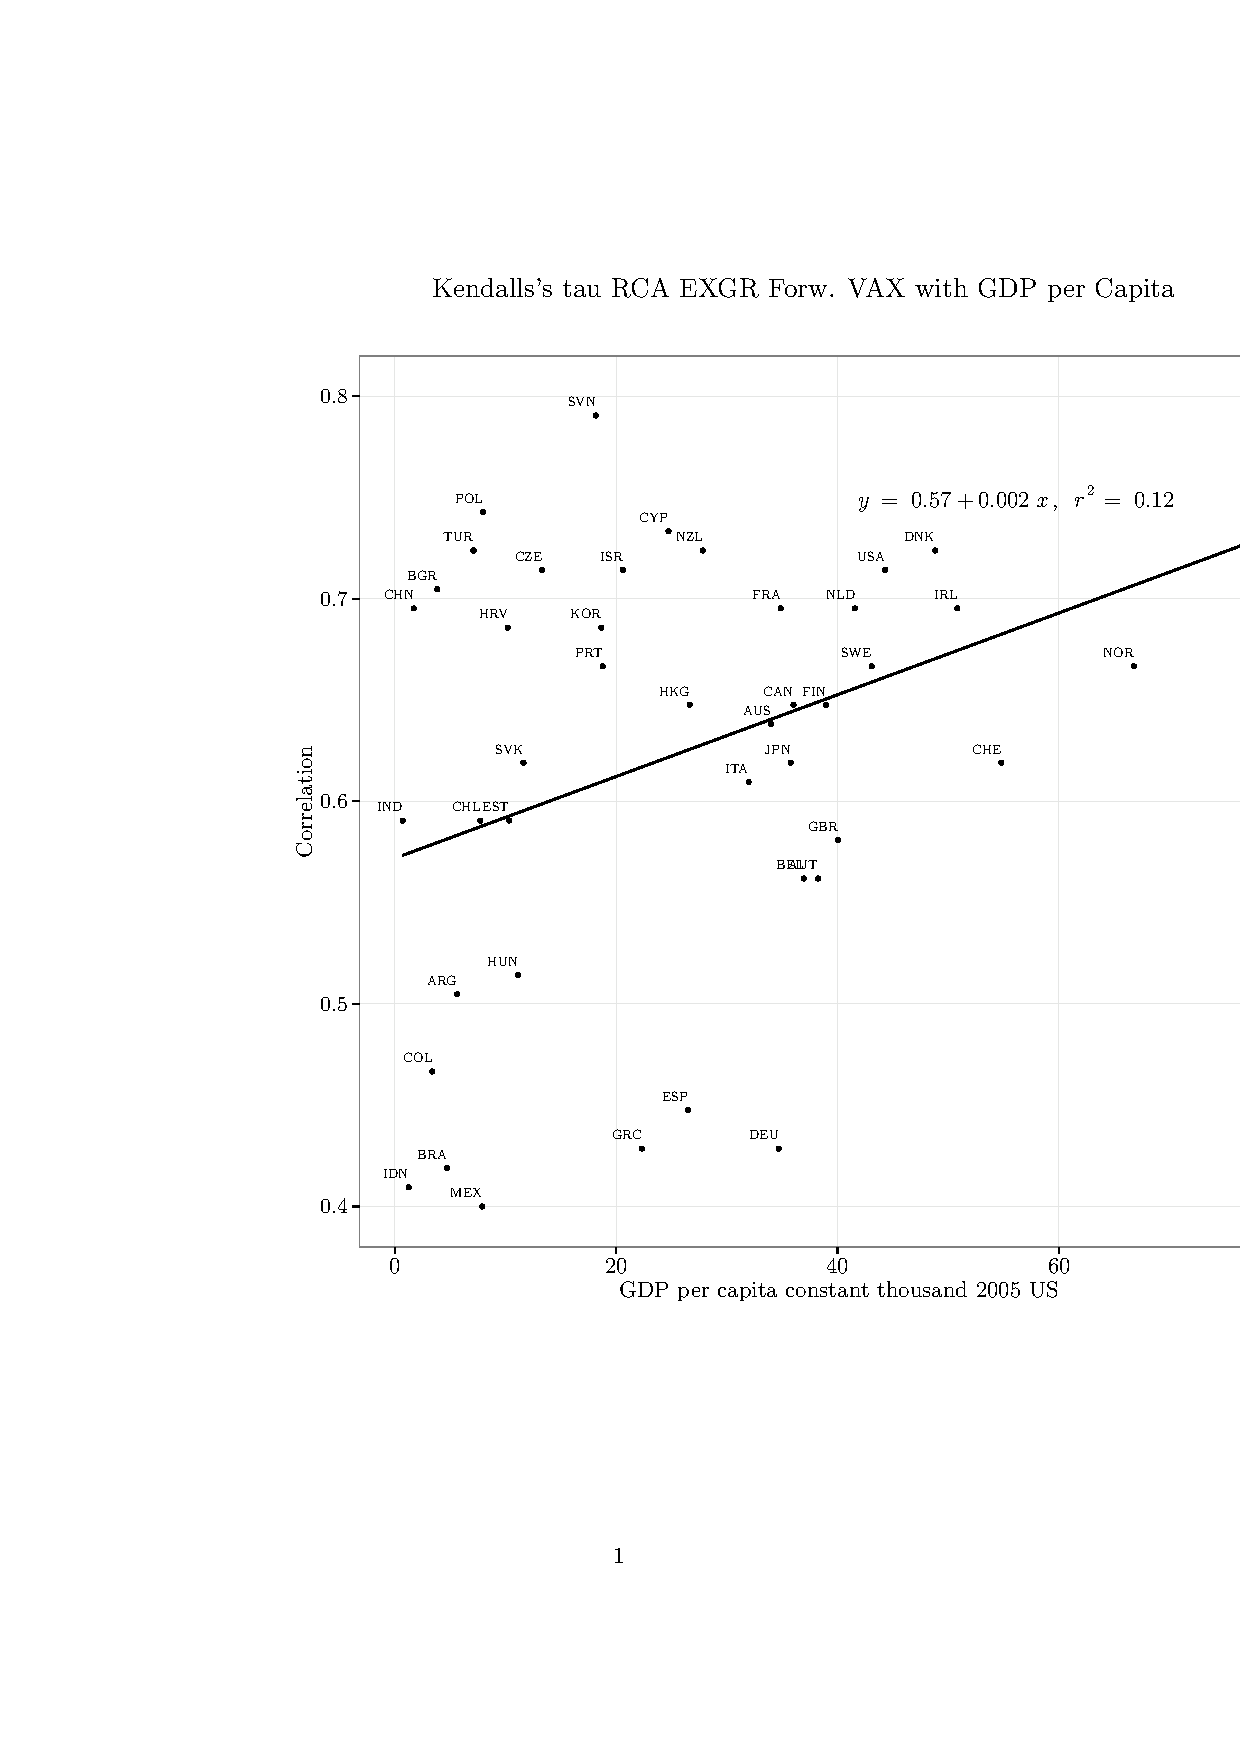
\includegraphics[width=.49\linewidth]{./fig/kendall_fddva_exgr_std_balassa-march.tex}
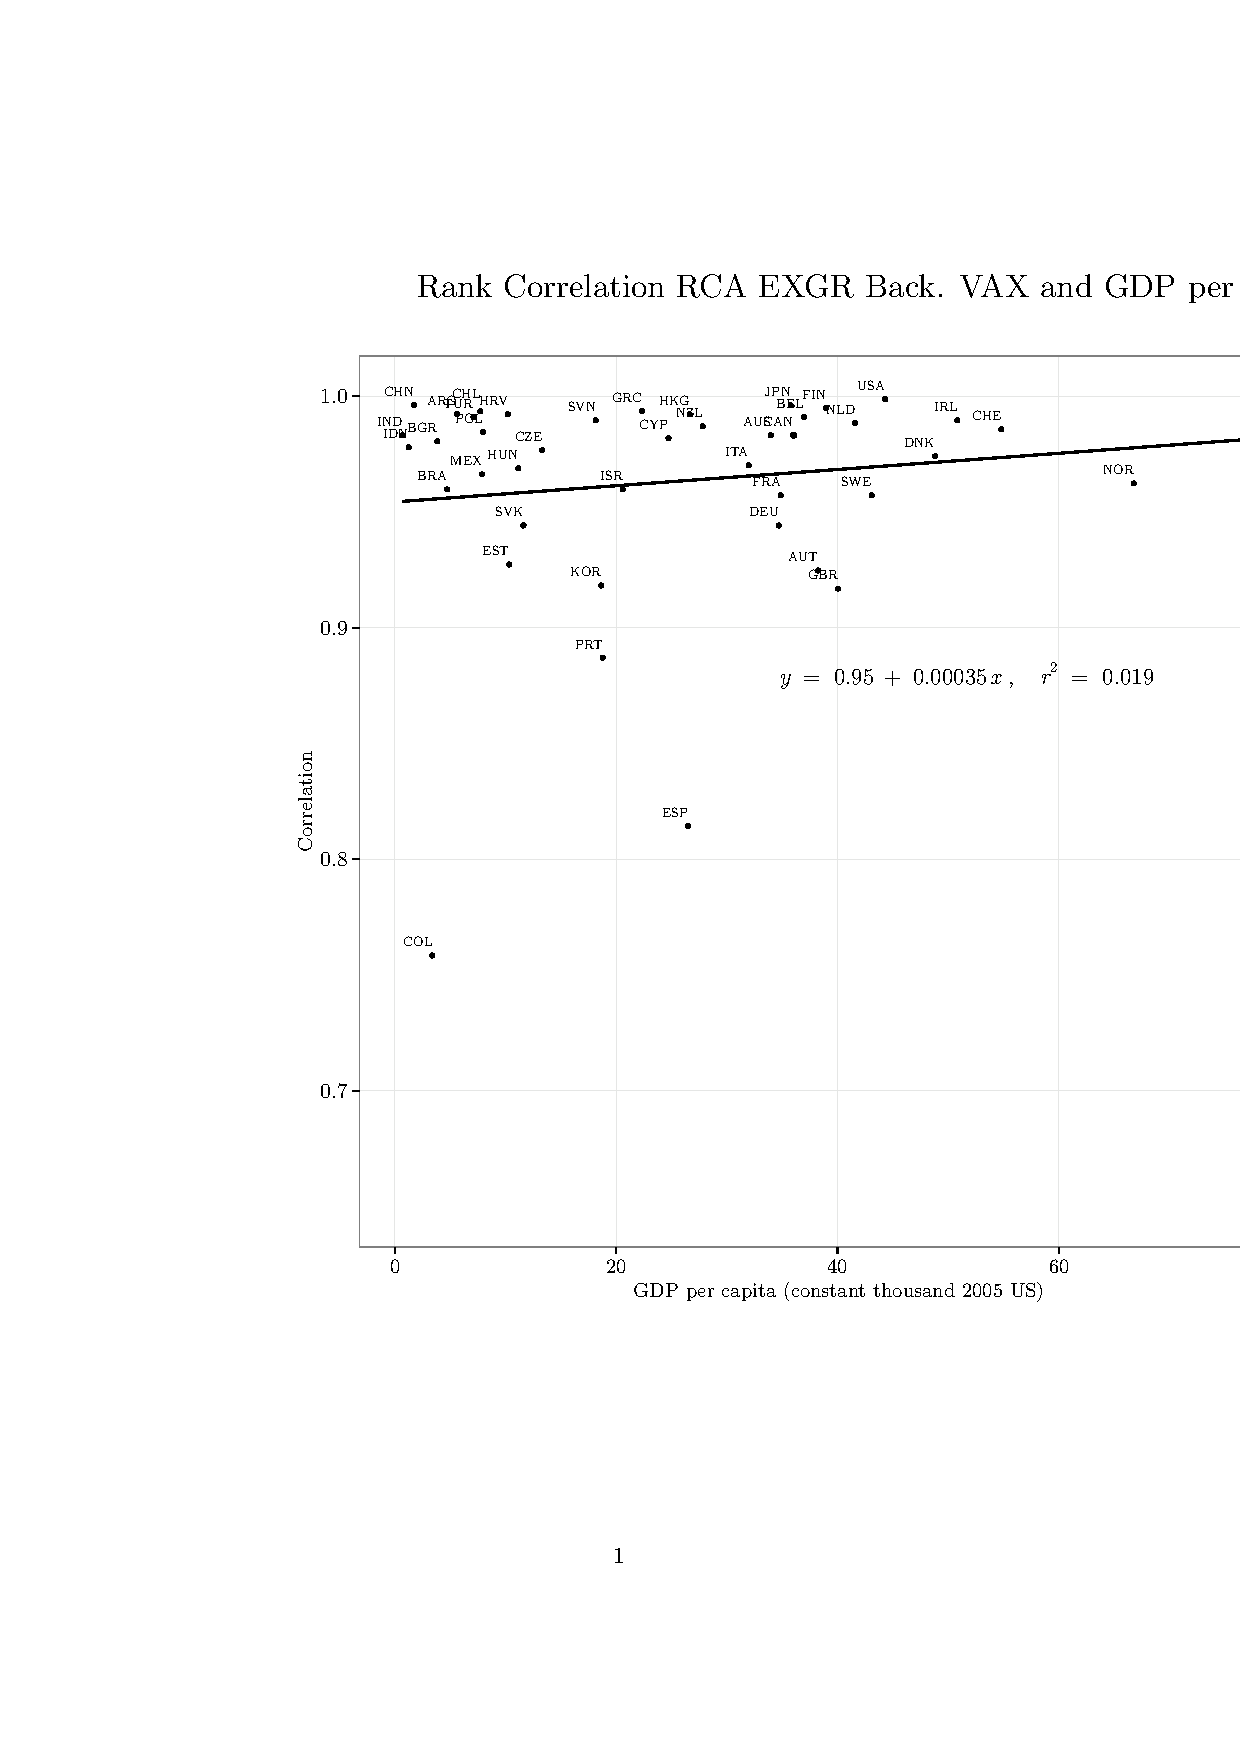
\includegraphics[width=.49 \linewidth]{./fig/spearman_exgr_dva_std_balassa-march.tex}
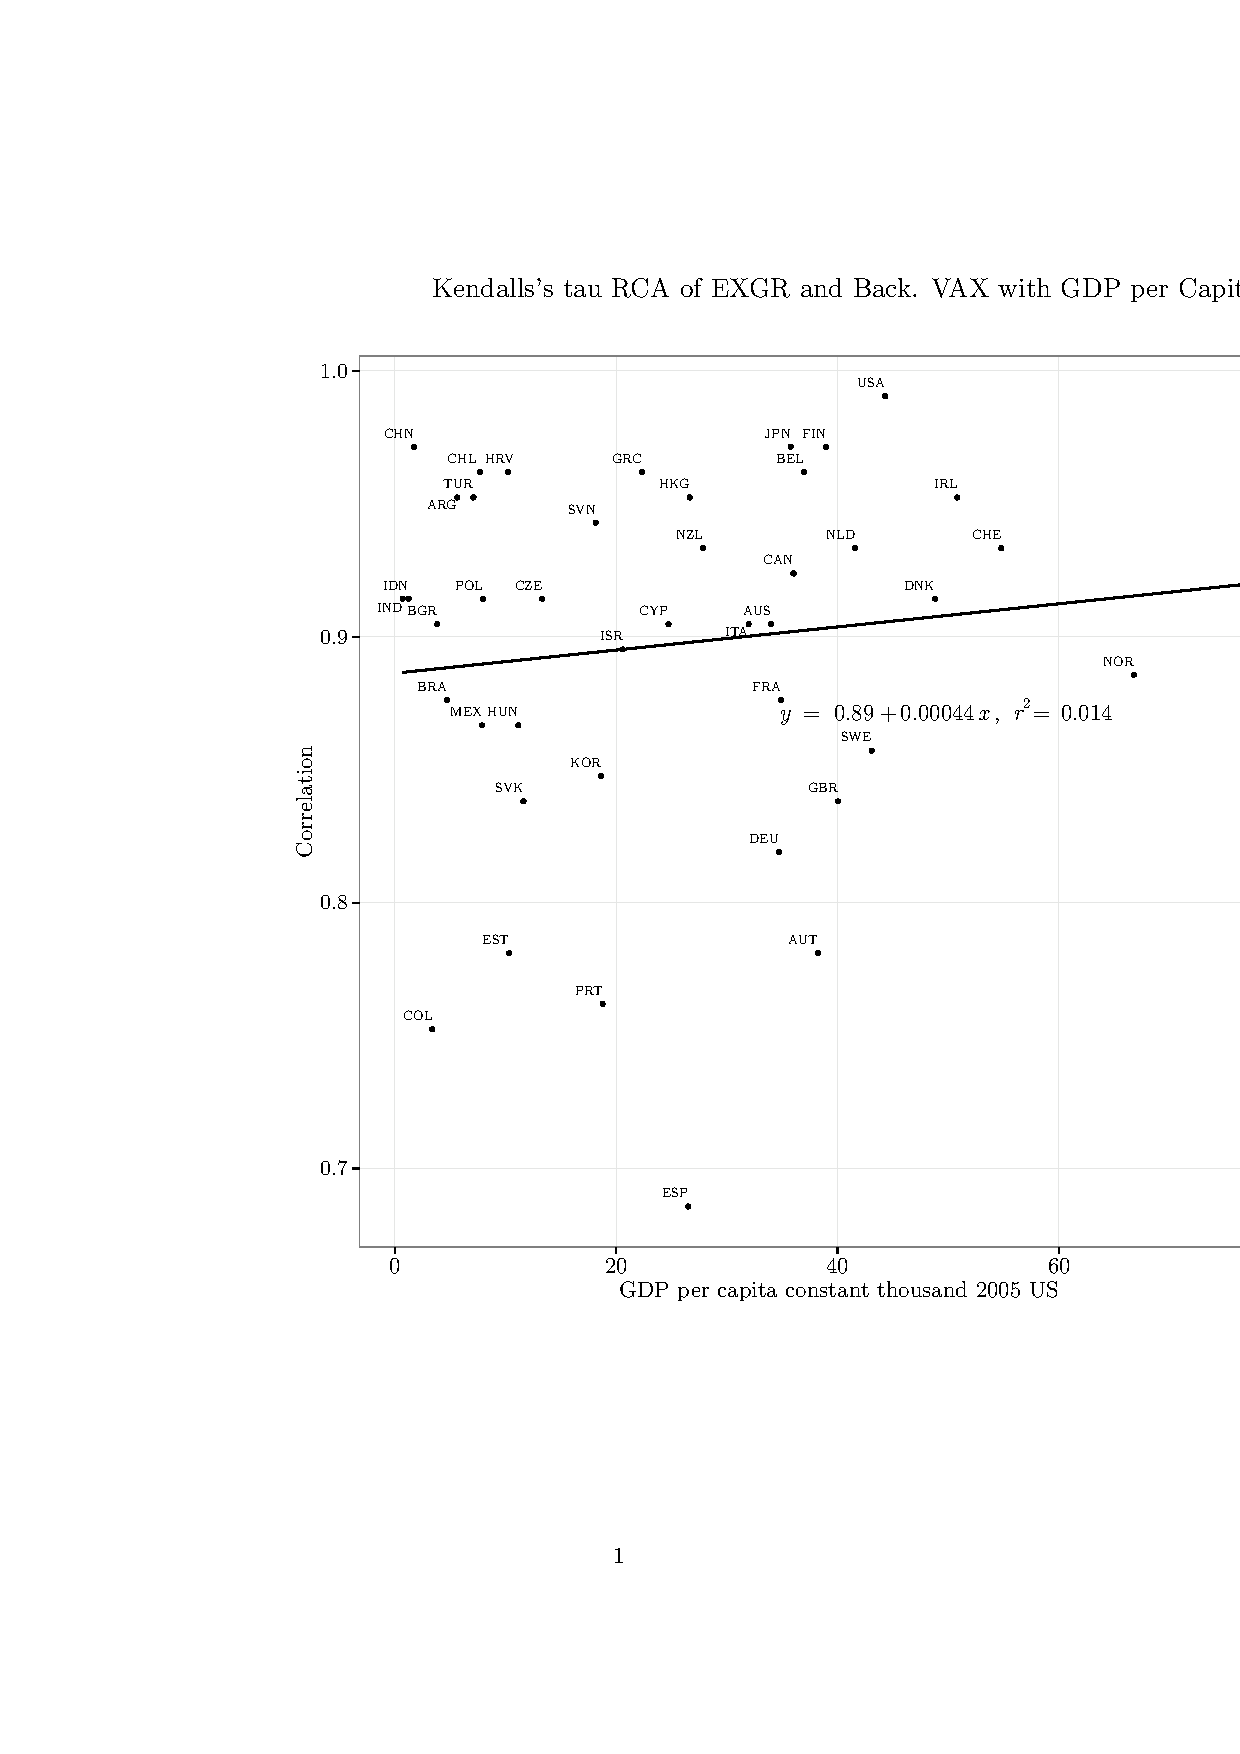
\includegraphics[width=.49\linewidth]{./fig/kendall_dva_exgr_std_balassa-march.tex}
 %\captionof{figure}{Another figure}
\end{figure}
I conclude four findings from the figures above.
Firstly, the RCA rankings based on gross exports and backward value-added exports show a high degree of similarity for all countries.
Secondly, the association between forward value-added exports and gross exports is substantially lower than the association of backward value-added and gross exports.
Thirdly,  the association of gross exports and forw. VAX shows a weak positive relation with a country's GDP per capita.
As a final point I observe that the overall strenght of the associations is higher using  Spearman's $\rho$ compared to Kendall's $\tau$. \par
The first and second finding are similar to the results in the estimation of the $\theta$ parameter.
The results showed that the estimates for backw. VAX and gross exports showed a similar pattern, while the estimates of forw. VAX were reduced and did not follow a pattern.
The third finding is consistent with the hypothesis that countries with a higher GDP have less sector specific input and sourcing patterns.
The forth finding is consistent with the result that asymptotically the ratio of the population analog of Spearman's $\rho$ and Kendall's $\tau$ is equal to three half \parencite{fredricks2007}. \par
Turning to the local view  I present below the normalized RCA based on both value-added export measures and gross exports for the industries of the manufacturing sector.
the RCA \footnote{ ormally, I define it as follows $RCA_{i}^{k}=\frac{ z^k_i * \bar{z} }{\bar{z}_i * \bar{z}^k}$, where $\bar{z}$ denotes the grand mean, $\bar{z}^k$ denotes the sector specific mean and $\bar{z}_i$ denotes the country specific mean.} as in \textcite{leromain2014}.
According to the normalization, an RCA  value above (below) 1 indicates a comparative (dis)advantage of a country in the particular industry.
 \par
To start with the RCA ranking results, I discuss the results for backward value-added exports and gross exports.
The major point which I conclude is that for both countries backward value added closely traces the RCA pattern of gross exports.
This results resembles the result of the estimation of $\theta$, where I observed a similar pattern. \par
The graph highlights that both countries highlights have an comparative advantage in the following sectors 20 23 24 26.
Germany has an higher comparative advantage in seven industries namely 20 21-22 25 27-28 29 30-33 34-35.
On the other hand, Belgium has an comparative advantage in six industries namely the food industry, 17-19 23 24 26 36-37.

 \par
In contrast, I observe that the RCA rankings are different for forward value-added gross exports.
Initially, I observe a largest decrease of RCA under forw. VAX compared to gross exports in the sector 23 and 20.
Additionally for Germany large decrease of RCA for the industry 21-22.
The largest decrease of RCA induces a change of 15\%  in the industry 23 for both countries.
As a result, the industry 23 changes from a comparative advatange to a comparative disadvantage for Germany.
The industry changes from an comparative advantage to comparative disadvantage, whereas for Belgium the industry remains a comparative advantage.
Additionally, in industry 20 both countries show no longer an comparative advantage under forw. VAX, whereas under gross exports they show an comparative advantage.
Moreover, I observe the largest increase of RCA under VAX compared to EXGR in the industry 29 and 30-33.
For both countries I observe an increase of about 5\% in the industry 30-33 for forw. VAX, and a somewhat smaller increase in the industry 29.
However, the pattern of RCA remains unchanged for both countries, for Belgium an comparative disadvantage and Germany has an comparative advantage.
Concluding, the graphs show that forward value-added exports changes the pattern of RCA, whereas backward value-added exports traces the pattern of RCA under gross exports.
 \begin{figure}
\caption{Country pair RCA based on for- and backward  VAX \& EXGR }
\includegraphics[width=.5\linewidth]{./fig/forw_exgr_DEU_BEL_tiva.tex}
\includegraphics[width=.5\linewidth]{./fig/back_exgr_DEU_BEL_tiva.tex}
\end{figure}

\endinput
